\documentclass[11pt,a4paper]{article}

% =============================================================================
% PACOTES BÁSICOS E CODIFICAÇÃO
% =============================================================================
\usepackage[utf8]{inputenc}
\usepackage[T1]{fontenc}
\usepackage[brazil]{babel}

% =============================================================================
% FORMATAÇÃO PADRÃO ABNT (NBR 14724 / NBR 6022 / NBR 10520 / NBR 6023)
% Margens: Superior e Esquerda = 3,0 cm; Inferior e Direita = 2,0 cm
% Espaçamento entre linhas: 1,5
% Recuo de parágrafo: 1,25 cm
% =============================================================================
\usepackage{geometry}
\geometry{
  a4paper,
  top=2.5cm,
  left=2.5cm,
  bottom=2cm,
  right=2cm
}

\usepackage{setspace}
\singlespacing

\usepackage{indentfirst}
\setlength{\parindent}{1.25cm}
\setlength{\parskip}{5.5pt plus 1.5pt minus 1pt}
\setlength{\headheight}{14.5pt}
\AtBeginDocument{%
  \setlength{\abovedisplayskip}{5pt plus 1.5pt minus 1.5pt}%
  \setlength{\belowdisplayskip}{5pt plus 1.5pt minus 1.5pt}%
  \setlength{\abovedisplayshortskip}{2.5pt plus 1pt minus 1pt}%
  \setlength{\belowdisplayshortskip}{2.5pt plus 1pt minus 1pt}%
  \setlength{\textfloatsep}{7pt plus 2pt minus 2pt}%
  \setlength{\floatsep}{5pt plus 2pt minus 2pt}%
  \setlength{\intextsep}{5pt plus 2pt minus 2pt}%
}

\makeatletter
\renewcommand
\section{\@startsection {section}{1}{\z@}%
  {-1.8ex \@plus -0.5ex \@minus -.2ex}%
  {0.8ex \@plus.2ex}%
{\normalfont\large\bfseries}}
\renewcommand
\subsection{\@startsection{subsection}{2}{\z@}%
  {-1.4ex\@plus -0.4ex \@minus -.2ex}%
  {0.6ex \@plus .2ex}%
{\normalfont\normalsize\bfseries}}
\renewcommand
\subsubsection{\@startsection{subsubsection}{3}{\z@}%
  {-1.0ex\@plus -0.3ex \@minus -.2ex}%
  {0.4ex \@plus .1ex}%
{\normalfont\normalsize\bfseries}}
\renewcommand\paragraph{\@startsection{paragraph}{4}{\z@}%
  {0.8ex \@plus0.2ex \@minus.1ex}%
  {-1em}%
{\normalfont\normalsize\bfseries}}
\makeatother

% Fonte serifada padrão (Times)
\usepackage{mathptmx}
\usepackage{microtype}

% Cabeçalho com numeração no canto superior direito (padrão ABNT)
\usepackage{fancyhdr}
\pagestyle{fancy}
\fancyhf{}
\fancyhead[R]{\footnotesize\thepage}
\renewcommand{\headrulewidth}{0pt}
\fancypagestyle{plain}{%
  \fancyhf{}%
  \fancyhead[R]{\footnotesize\thepage}%
  \renewcommand{\headrulewidth}{0pt}%
}

% =============================================================================
% PACOTES MATEMÁTICOS, GRÁFICOS E ELEMENTOS FLUTUANTES
% =============================================================================
\usepackage{amsmath}
\usepackage{amssymb}
\usepackage{amsfonts}
\usepackage{amsthm}
\usepackage{mathtools}

\usepackage{graphicx}
\graphicspath{{Imagens/}}

\usepackage{float}
\usepackage{booktabs}
\usepackage{array}
\usepackage{caption}
\usepackage{subcaption}
\usepackage{xcolor}
\usepackage{enumitem}
\setlist{itemsep=2.5pt, topsep=3.5pt, parsep=0pt, partopsep=0pt, leftmargin=*}
\usepackage[hyperfootnotes=true]{hyperref}

\captionsetup{
  font=footnotesize,
  labelfont=bf,
  labelsep=endash
}

\hypersetup{
  colorlinks=true,
  breaklinks=true,
  linkcolor=blue!75!black,
  citecolor=black,
  urlcolor=blue!75!black,
  pdftitle={Leilões como Jogos Bayesianos: Lances, Maldição do
  Vencedor e Equivalência de Receita},
  pdfauthor={João Matheus Alves Lima, Lucas Ulrich Rafagnin, Mateus
  Fernandes Araujo, Pedro Ulisses de Lima Quadros, Thiago Henrique Bueno}
}

% Torna o número da chamada de nota de rodapé azul, em negrito e entre colchetes para alta visibilidade
\makeatletter
\renewcommand{\@makefnmark}{\hbox{\@textsuperscript{\normalfont\bfseries\textcolor{blue!80!black}{[\@thefnmark]}}}}
\makeatother

% =============================================================================
% CONFIGURAÇÃO DE CITAÇÃO ABNT (AUTOR, ANO) COM THEBIBLIOGRAPHY MANUAL
% Faz com que \cite{label} imprima (AUTOR, ANO) conforme NBR 10520
% =============================================================================
\makeatletter
\def\@cite#1#2{(#1\if@tempswa , #2\fi)}
\def\@citex[#1]#2{\leavevmode
  \let\@citea\@empty
  \@cite{\@for\@citeb:=#2\do
    {\@citea\def\@citea{;\penalty\@m\ }%
      \edef\@citeb{\expandafter\@firstofone\@citeb\@empty}%
      \if@filesw\immediate\write\@auxout{\string\citation{\@citeb}}\fi
      \@ifundefined{b@\@citeb}{\hbox{\reset@font\bfseries ?}%
        \G@refundefinedtrue
        \@latex@warning
      {Citation `\@citeb' on page \thepage \space undefined}}%
{\csname b@\@citeb\endcsname}}}{#1}}
\def\@biblabel#1{}
\renewenvironment{thebibliography}[1]
{\list{\@biblabel{\@arabic\c@enumiv}}%
  {\settowidth\labelwidth{}%
    \leftmargin 0pt
    \itemindent 0pt
    \parsep 2pt
    \itemsep 2pt
    \@openbib@code
    \usecounter{enumiv}%
    \let\p@enumiv\@empty
  \renewcommand\theenumiv{\@arabic\c@enumiv}}%
  \singlespacing
  \raggedright
  \sloppy
  \clubpenalty4000
  \@clubpenalty \clubpenalty
  \widowpenalty4000%
\sfcode`\.\@m}
{\def\@noitemerr
  {\@latex@warning{Empty `thebibliography' environment}}%
\endlist}
\makeatother

% =============================================================================
% AMBIENTES FORMAIS PARA TEORIA DOS JOGOS
% =============================================================================
\newtheoremstyle{compactdef}{5.5pt}{5.5pt}{\normalfont}{}{\bfseries}{.}{0.5em}{}
\newtheoremstyle{compactthm}{5.5pt}{5.5pt}{\itshape}{}{\bfseries}{.}{0.5em}{}
\theoremstyle{compactdef}
\newtheorem{definicao}{Definição}[section]
\newtheorem{exemplo}{Exemplo}[section]

\theoremstyle{compactthm}
\newtheorem{teorema}{Teorema}[section]
\newtheorem{proposicao}{Proposição}[section]
\newtheorem{lema}{Lema}[section]
\newtheorem{corolario}{Corolário}[section]

\theoremstyle{remark}
\newtheorem{observacao}{Observação}[section]

% Ambiente para citação direta longa (> 3 linhas) conforme ABNT NBR 10520
% Recuo de 4 cm da margem esquerda, espaçamento simples e fonte menor (10pt)
\newenvironment{citacaoabnt}{%
  \par\vspace{0.25cm}%
  \begin{singlespace}%
    \footnotesize%
    \list{}{%
      \setlength{\leftmargin}{4cm}%
      \setlength{\rightmargin}{0cm}%
      \setlength{\topsep}{0pt}%
      \setlength{\partopsep}{0pt}%
      \setlength{\parsep}{0pt}%
    }%
  \item\relax
  }{%
    \endlist%
  \end{singlespace}%
  \vspace{0.25cm}\par%
}

% =============================================================================
% CORPO DO DOCUMENTO
% =============================================================================
\begin{document}

\thispagestyle{empty}
\begin{center}
  {\normalsize \textbf{INSTITUTO TECNOLÓGICO DE AERONÁUTICA (ITA)}}\\
  {\small Disciplina: GED-62 -- Teoria dos Jogos \quad|\quad
  Professor: Darcton Damião}\\[0.2cm]
  {\large \textbf{LEILÕES COMO JOGOS BAYESIANOS: LANCES, MALDIÇÃO DO
  VENCEDOR E EQUIVALÊNCIA DE RECEITA}}\\[0.15cm]
  {\normalsize \textbf{Grupo 5}}\\[0.05cm]
  {\small João Matheus Alves Lima $\cdot$ Lucas Ulrich Rafagnin
  $\cdot$ Mateus Fernandes Araujo}\\
  {\small Pedro Ulisses de Lima Quadros \textit{(Ponto Focal)}
  $\cdot$ Thiago Henrique Bueno}\\[0.1cm]
  {\small São José dos Campos -- SP, Novembro de 2026}
\end{center}
\vspace{0.1cm}

% Resumo no padrão ABNT NBR 6022 (espaçamento simples no resumo)
\begin{singlespace}
  \footnotesize
  \noindent\textbf{Resumo:} Este artigo apresenta a teoria dos
  leilões sob a perspectiva dos jogos bayesianos (jogos de informação
  incompleta). Partindo dos conceitos de tipo privado, distribuição
  de crenças a priori (\textit{prior} comum), estratégia funcional e
  Equilíbrio de Nash Bayesiano (ENB), contrastamos os ambientes de
  Valores Privados Independentes e de Valor Comum e analisamos os
  quatro formatos clássicos de leilão (Inglês, Holandês, Primeiro
  Preço e Segundo Preço de Vickrey). Demonstramos por que a revelação
  sincera ($b_i = v_i$) é fracamente dominante no segundo preço, por
  que o sombreamento de lance (\textit{bid shading}, $b_i < v_i$) é
  obrigatório no primeiro preço, e como ambos geram a mesma receita
  esperada pelo Teorema da Equivalência de Receita, além de
  explicarmos a Maldição do Vencedor sob valor comum. Em seguida,
  resolvemos passo a passo o leilão de primeiro preço com dois
  jogadores e valores uniformes em $[0,1]$, validando a equivalência
  de receita ($\mathbb{E}[R] = 1/3$) com uma simulação de $10.000$
  leilões em Python. Por fim, modelamos o caso real dos leilões de
  anúncios online (Google Ads e \textit{Ad Exchanges}), explicando a
  mudança de 2002 do 1º para o 2º preço e o retorno de 2019 ao 1º
  preço com \textit{Header Bidding}.

  \vspace{0.1cm}
  \noindent\textbf{Palavras-chave:} Teoria dos Jogos. Jogos
  Bayesianos. Leilões. Equivalência de Receita. Maldição do Vencedor.
\end{singlespace}

\vspace{0.2cm}

% =============================================================================
% IMPORTAÇÃO DAS SEÇÕES MODULARES
% =============================================================================
\section{Introdução}
\label{sec:introducao}

A alocação de bens, contratos e recursos escassos quando o vendedor desconhece quanto cada comprador está disposto a pagar é um dos problemas mais importantes da economia e da engenharia. Na prática, leilões movimentam trilhões de dólares anualmente: governos leiloam frequências de telecomunicações (como o 5G), campos de petróleo e concessões de energia, enquanto plataformas digitais como o Google realizam bilhões de leilões instantâneos todos os dias para vender espaços de anúncios na internet \cite{klemperer2004,edelman2007,despotakis2021}.

Do ponto de vista da Teoria dos Jogos, um leilão difere dos jogos clássicos de informação completa (como o Dilema dos Prisioneiros ou o xadrez) porque envolve \textbf{informação incompleta}: cada participante sabe quanto o objeto vale para si, mas desconhece o quanto ele vale para os seus concorrentes. Até a década de 1960, não se sabia como calcular um Equilíbrio de Nash nesse cenário sem cair em uma regressão infinita de crenças. Esse problema foi resolvido pelos trabalhos clássicos de \cite{vickrey1961} e \cite{harsanyi1967} (laureados com o Prêmio Nobel), que modelaram os leilões como \textbf{jogos bayesianos} por meio dos conceitos de \textit{Tipo Privado} e de \textit{Prior Comum} \cite{gibbons1992}.

Neste artigo, apresentamos de forma construtiva e acessível a teoria dos leilões como jogos bayesianos. Na Seção~\ref{sec:conceito}, definimos sequencialmente os conceitos fundamentais (tipos, \textit{prior} comum, estratégias funcionais, Equilíbrio de Nash Bayesiano, valores privados vs. valores comuns, os quatro formatos clássicos de leilão, o Teorema da Equivalência de Receita e a Maldição do Vencedor). Na Seção~\ref{sec:modelo_resolvido}, resolvemos passo a passo o leilão de primeiro preço com dois participantes e valores uniformes em $[0,1]$, comparando sua receita com a do leilão de segundo preço. Na Seção~\ref{sec:caso_real}, analisamos e modelamos o caso real dos leilões de anúncios online (Google Ads e \textit{Ad Exchanges}). Por fim, a Seção~\ref{sec:ligacao_curso} conecta o tema à disciplina GED-62 e a Seção~\ref{sec:conclusao} apresenta as conclusões.

\section{Conceito}
\label{sec:conceito}

Para apresentar a teoria dos leilões como uma construção lógica clara --- sem depender de formalismo excessivo ---, definimos explicitamente cada termo antes de utilizá-lo no passo seguinte.

\subsection{Leilões como Jogos Bayesianos}
\label{subsec:jogos_bayesianos}

\begin{definicao}[Jogo de Informação Completa]
\label{def:info_completa}
É um jogo em que todos os jogadores conhecem perfeitamente quem são os participantes, quais ações cada um pode tomar e \textbf{quanto cada jogador ganha (\textit{payoff}) em qualquer combinação de ações}. Não há segredo sobre os objetivos, custos ou avaliações dos adversários \cite{gibbons1992}.
\end{definicao}

No \textit{Dilema dos Prisioneiros}, por exemplo, o Prisioneiro~A sabe exatamente quantos anos de pena o Prisioneiro~B recebe em cada célula da matriz. Porém, em um leilão real, a informação completa não existe: quem disputa um imóvel ou uma concessão pública sabe quanto o bem vale para si, mas \textbf{não sabe quanto ele vale para o seu concorrente}. Isso nos leva à segunda definição:

\begin{definicao}[Jogo de Informação Incompleta / Jogo Bayesiano]
\label{def:jogo_bayesiano}
É um jogo no qual pelo menos um jogador desconhece a função de \textit{payoff} (o ganho líquido) de outro jogador, porque esse ganho depende de informações privadas que só o outro jogador conhece \cite{harsanyi1967,gibbons1992}.
\end{definicao}

Até a década de 1960, os economistas acreditavam ser impossível aplicar o Equilíbrio de Nash a jogos de informação incompleta: para saber minha melhor jogada, preciso prever a jogada do adversário, que depende do \textit{payoff} secreto dele; logo, eu teria que estimar o que acho do \textit{payoff} dele, e o que ele acha que eu acho do \textit{payoff} dele, gerando uma regressão infinita de crenças. \cite{vickrey1961} e \cite{harsanyi1967} resolveram esse impasse por meio da \textbf{Transformação de Harsanyi}, baseada nos conceitos de \textbf{Tipo Privado} e \textbf{\textit{Prior} Comum}:

\begin{definicao}[Tipo Privado ($\theta_i$)]
\label{def:tipo_privado}
É o pedaço de informação secreta que pertence exclusivamente ao jogador $i$ e que determina o seu \textit{payoff}. Nos leilões, o \textbf{tipo} de um comprador nada mais é do que a sua informação privada sobre o valor do objeto (o máximo que ele estaria disposto a pagar, ou a estimativa técnica que a sua equipe fez sobre o bem).
\end{definicao}

Por exemplo, se duas construtoras disputam uma licitação para erguer uma ponte, e a Construtora~1 (com máquinas novas) faz a obra por R\$\,80 milhões enquanto a Construtora~2 (com máquinas antigas) gasta R\$\,95 milhões, esse custo interno secreto é o \textbf{Tipo ($\theta_i$)} de cada uma: cada empresa vê a sua própria planilha, mas não vê a da concorrente. Como então tomar uma decisão racional?

\begin{definicao}[Distribuição de Crenças a Priori / \textit{Prior} Comum $F$]
\label{def:prior_comum}
É a distribuição conjunta de probabilidade $F(\theta_1, \theta_2, \dots, \theta_n)$ segundo a qual a ``Natureza'' sorteia os \textbf{Tipos} de todos os jogadores antes de o jogo começar, sendo essa regra estatística de sorteio conhecida por todos os participantes \cite{harsanyi1967,gibbons1992}.
\end{definicao}

Vale esclarecer três pontos sobre o \textit{Prior} Comum $F$:
\begin{enumerate}[label=\arabic*.]
    \item \textbf{Origem do termo \textit{Prior}:} Vem da Estatística Bayesiana (\textit{a priori}, em oposição a \textit{a posteriori}). Harsanyi propôs imaginar que o jogo começa um passo antes, com um jogador fictício chamado \textbf{Natureza}: no estágio inicial (\textit{ex ante}), a Natureza gira uma roleta probabilística $F$ e sorteia um cartão secreto com o Tipo $\theta_i$ para cada jogador $i$ (\textit{Prior}); em seguida (\textit{estágio interim}), cada jogador espia apenas o seu próprio cartão $\theta_i$ e atualiza suas probabilidades usando a Regra de Bayes.
    \item \textbf{Por que se chama ``Comum''?} ``Prior Comum'' \textbf{não} significa que todos os jogadores são sorteados da mesma curva estatística. Vem de \textit{Conhecimento Comum} (\textit{Common Knowledge}): todos os jogadores da mesa conhecem e concordam sobre quais são as regras da roleta da Natureza ($F$).
    \item \textbf{Simetria, Assimetria e Correlação:} Dentro da lei geral $F(\theta_1, \dots, \theta_n)$, ocorrem três casos práticos: (a) \textit{Distribuição Universal / Jogadores Simétricos ($F_1 = \dots = F_n$)}, como dois estudantes disputando um ingresso com valores sorteados entre R\$\,0 e R\$\,100 (caso da Seção~\ref{sec:modelo_resolvido}); (b) \textit{Distribuição Particular / Jogadores Assimétricos ($F_1 \neq F_2$)}, como num leilão do 5G em que o valor de uma grande operadora sai de $[500, 1000]$ milhões ($F_1$) e o de uma provedora regional sai de $[100, 400]$ milhões ($F_2$), sendo ambas as curvas conhecidas por todos; e (c) \textit{Tipos Correlacionados}, como no pôquer, em que o baralho de 52 cartas é o mesmo \textit{Prior} inicial para todos, mas após cada jogador olhar suas cartas ($\theta_i$), cada um passa a ter uma distribuição condicional (\textit{posterior} $F(\theta_{-i} \mid \theta_i)$) diferente.
\end{enumerate}

Na notação da Teoria dos Jogos, o subscrito \textbf{``$-i$''} (``todos exceto $i$'') indica o vetor dos concorrentes de $i$: $\theta_{-i} = (\theta_1, \dots, \theta_{i-1}, \theta_{i+1}, \dots, \theta_n)$ e $b_{-i} = (b_1, \dots, b_{i-1}, b_{i+1}, \dots, b_n)$ (com 2 jogadores, $\theta_{-1} = \theta_2$ e $b_{-1} = b_2$). Com isso, definimos estratégia e equilíbrio:

\begin{definicao}[Estratégia em um Jogo Bayesiano ($b_i(\theta_i)$)]
\label{def:estrategia_bayesiana}
Em um jogo bayesiano, uma estratégia \textbf{não é uma única ação isolada}, mas sim um \textbf{plano completo (uma função matemática)} que especifica qual ação (lance) o jogador $i$ escolherá \textbf{para cada Tipo $\theta_i$ que a Natureza possa ter sorteado para ele} \cite{gibbons1992}.
\end{definicao}

A estratégia precisa ser uma função porque o Jogador~1 (que tirou, digamos, $v_1 = 80$) não sabe qual valor $v_2$ o Jogador~2 tirou hoje ($10$, $50$ ou $90$); logo, ele só consegue calcular a probabilidade de vencer se souber a \textbf{regra (função)} $b_2(v_2)$ que o Jogador~2 usa para converter qualquer valor $v_2$ em um lance (por exemplo, $b_2(v_2) = 0{,}5\,v_2$).

\begin{definicao}[Equilíbrio de Nash Bayesiano --- ENB]
\label{def:enb}
É um perfil de funções de estratégia ($b_1^*(\theta_1),$ $\dots,$ $b_n^*(\theta_n)$) --- uma regra de lance para cada jogador --- tal que, para todo jogador $i$ e para todo Tipo possível $\theta_i$ desse jogador, o lance $b_i^*(\theta_i)$ maximiza o \textbf{ganho médio esperado} de $i$ (calculado sobre a distribuição de tipos dos adversários $F(\theta_{-i} \mid \theta_i)$), dado que todos os outros jogadores estão usando as funções de lance $b_{-i}^*(\theta_{-i})$.
\end{definicao}

Destacamos duas propriedades importantes do ENB: (i) a função $b_i^*(\theta_i)$ atinge o ganho máximo para \textit{qualquer tipo próprio $\theta_i$} (pois o jogador já conhece seu próprio tipo ao dar o lance), mas apenas \textit{na média esperada (\textit{interim})} sobre os tipos dos outros $\theta_{-i}$ (no 1º preço, $b^*(v_i) = v_i/2$ é ótimo em média antes de abrir os envelopes; já no 2º preço de Vickrey, a estratégia sincera $b^*(v_i) = v_i$ é ainda mais forte, pois é ótima para \textit{qualquer combinação realizada $(v_1, v_2)$}, constituindo um Equilíbrio em Estratégias Dominantes / \textit{Ex Post}); e (ii) no ENB, todos conhecem a \textbf{função (fórmula)} dos adversários (como uma ``calculadora de vidro transparente'' programada para dividir por 2), mas o segredo está no \textbf{número $v_j$} que cada adversário digitou na calculadora hoje.

% =============================================================================
\subsection{Valores Privados e Valores Comuns}
\label{subsec:valores_privados_comuns}

\begin{definicao}[Valoração ($v_i$) e Excedente / \textit{Payoff} ($u_i$)]
\label{def:valoracao_payoff}
A \textbf{Valoração ($v_i$)} é o valor monetário máximo que o objeto leiloado tem para o jogador $i$ (sua disposição máxima a pagar). Se o jogador $i$ vence o leilão e paga um preço $p$, o seu ganho líquido (\textbf{Excedente do Comprador} ou \textbf{\textit{Payoff}}) é $u_i = v_i - p$. Se perde o leilão e não paga nada, seu \textit{payoff} é $u_i = 0$.
\end{definicao}

Na literatura de leilões, há dois ambientes clássicos que relacionam a Valoração $v_i$ com o Tipo $\theta_i$ \cite[p.~13--14]{klemperer2004}:

\begin{definicao}[Modelo de Valores Privados Independentes --- IPV (\textit{Independent Private Values})]
\label{def:ipv}
É o ambiente de leilão em que: (1) \textbf{Valor Privado ($v_i = \theta_i$):} cada jogador $i$ conhece com $100\%$ de certeza qual é a sua própria Valoração $v_i$ antes do leilão começar; mesmo que ele descobrisse o Tipo dos concorrentes, isso \textbf{não mudaria em um centavo} o quanto o objeto vale para ele; e (2) \textbf{Independência Estatística:} o valor $v_i$ de um jogador foi sorteado de forma independente do valor $v_j$ dos outros jogadores.
\end{definicao}

Um exemplo de Valor Privado é o leilão de uma camisa autografada do time de coração (para uso próprio, sem revenda): se ela vale R\$\,500 para você, descobrir que seu vizinho daria apenas R\$\,20 porque torce para outro time não altera o fato de que ela continua valendo R\$\,500 para você.

\begin{definicao}[Modelo de Valor Comum Puro --- CV (\textit{Common Value})]
\label{def:cv}
É o ambiente de leilão em que o objeto tem \textbf{exatamente o mesmo valor final objetivo $V$ para todos os participantes} ($v_1 = v_2 = \dots = v_n = V$), mas \textbf{ninguém conhece o valor verdadeiro $V$ no momento do leilão}. O Tipo de cada jogador ($\theta_i = s_i$) é apenas um \textbf{Sinal Privado} (uma estimativa com margem de erro, $s_i = V + \varepsilon_i$) sobre o verdadeiro valor $V$. Nesse ambiente, se um jogador descobrisse o Sinal Privado dos concorrentes, ele \textbf{mudaria imediatamente a sua própria estimativa} de quanto o objeto vale!
\end{definicao}

O exemplo clássico de Valor Comum é o leilão de um bloco de petróleo no pré-sal: a quantidade física de óleo no subsolo ($V$) é uma só para qualquer petroleira que vença, mas cada empresa tem apenas o laudo sísmico do seu próprio geólogo ($s_i$) \cite[p.~13--14]{klemperer2004}. Se o geólogo da Empresa~1 estimou US\$\,1,2~bi, mas ela descobre que os geólogos de duas concorrentes estimaram apenas US\$\,0,8~bi e US\$\,0,7~bi, a Empresa~1 percebe na hora que seu geólogo foi otimista demais e revê sua avaliação para baixo.

% =============================================================================
\subsection{Leilões de Primeiro Preço e de Segundo Preço (Vickrey)}
\label{subsec:formatos_leilao}

A Tabela~\ref{tab:quatro_formatos} resume os quatro formatos clássicos de leilão \cite{vickrey1961,klemperer2004}.

\begin{table}[htbp]
\centering
\caption{Os quatro formatos clássicos de leilão de um único objeto.}
\label{tab:quatro_formatos}
\footnotesize
\begin{tabular}{p{4.3cm} p{10.5cm}}
\toprule
\textbf{Formato de Leilão} & \textbf{Como Funciona (Regra de Alocação e Pagamento)} \\
\midrule
\textbf{1. Ascendente Aberto (Inglês)} & O preço começa baixo e vai subindo. Os participantes vão saindo até sobrar apenas um, que vence e paga o preço em que o penúltimo desistiu. \\
\textbf{2. Descendente Aberto (Holandês)} & O preço começa alto em um relógio e vai caindo. O primeiro participante que gritar ``Pare!'' vence imediatamente e paga o preço mostrado no relógio. \\
\textbf{3. 1º Preço em Envelope Fechado} & Cada participante entrega um lance secreto $b_i$ num envelope. Quem deu o maior lance vence e \textbf{paga o valor do seu próprio lance ($b_i$)}. \\
\textbf{4. 2º Preço em Envelope Fechado (Vickrey)} & Cada participante entrega um lance secreto $b_i$ num envelope. Quem deu o maior lance vence, mas \textbf{paga o valor do segundo maior lance} entregue pelos concorrentes. \\
\bottomrule
\end{tabular}
\par\vspace{0.05cm}
{\footnotesize Fonte: Elaborado pelos autores com base em \cite{vickrey1961} e \cite[p.~11--12]{klemperer2004}.}
\end{table}

No \textbf{Leilão Inglês}, a disputa pode ocorrer tanto com os participantes gritando lances crescentes (\textit{open-outcry}) quanto com um relógio subindo continuamente a partir de R\$\,0, onde todos começam de mão levantada e cada um abaixa a mão ao atingir seu limite, travando o relógio quando o penúltimo desiste \cite[p.~11]{klemperer2004}. Por exemplo, se um quadro vale $v_{\text{Ana}} = 50$, $v_{\text{Lucas}} = 80$ e $v_{\text{João}} = 100$, Ana desiste em R\$\,50 e Lucas desiste em R\$\,80; em ambas as modalidades, João vence pagando R\$\,80 (ou R\$\,80,01) sem precisar revelar que chegaria até R\$\,100. Daí decorrem duas equivalências fundamentais \cite[p.~20]{vickrey1961}:
\begin{enumerate}[label=\arabic*.]
    \item \textbf{Leilão Holandês $\equiv$ Leilão de 1º Preço (Sempre equivalentes):} No holandês, ninguém observa nada até alguém apertar o botão e encerrar o jogo; logo, escolher o número de parada no relógio e pagar esse próprio número é idêntico a escrevê-lo num envelope fechado de 1º preço.
    \item \textbf{Leilão Inglês $\equiv$ Leilão de 2º Preço / Vickrey (Equivalentes sob Valores Privados):} No inglês com valores privados, cada participante fica ativo até seu valor $v_i$; quando o penúltimo desiste no segundo maior valor da sala, o detentor do maior valor vence pagando o valor do segundo colocado --- exatamente a regra de Vickrey.
\end{enumerate}

Analisemos agora as duas estratégias centrais nos formatos de envelope fechado:

\begin{definicao}[Sombreamento de Lance --- \textit{Bid Shading}]
\label{def:bid_shading}
É o ato deliberado de submeter um lance \textbf{estritamente menor do que a sua verdadeira Valoração} ($b_i < v_i$).
\end{definicao}

Por que o \textit{Bid Shading} é obrigatório no \textbf{Leilão de 1º Preço}? Pela fórmula do \textbf{Valor Esperado do Ganho (\textit{Payoff} Esperado)} do jogador $i$:
\begin{equation}
\label{eq:payoff_esperado_1p}
\mathbb{E}[u_i(b_i) \mid v_i] = \underbrace{(v_i - b_i)}_{\text{Lucro se vencer}} \times \underbrace{\mathbb{P}\!\Big(b_i > \max_{j \neq i} b_j\Big)}_{\text{Probabilidade de vencer}} + \underbrace{0 \times \mathbb{P}\!\Big(b_i < \max_{j \neq i} b_j\Big)}_{\text{Ganho se perder } (=0)}.
\end{equation}
Se o jogador escrever seu valor verdadeiro no envelope ($b_i = v_i$), o primeiro termo $(v_i - v_i)$ zera e seu ganho esperado é \textbf{zero}! Para ter ganho esperado positivo, todo jogador racional precisa fazer \textit{bid shading} ($b_i < v_i$), equilibrando o \textit{trade-off}: subir o lance aumenta a probabilidade de vencer, mas reduz a margem $(v_i - b_i)$; baixar o lance aumenta a margem, mas reduz a chance de vitória. No Equilíbrio de Nash Bayesiano, o lance ótimo sombreado resulta exatamente no \textbf{Valor Esperado do maior adversário, condicionado a todos os adversários terem valor menor que $v_i$}:
\begin{equation}
\label{eq:lance_otimo_1p_esperanca}
b_{\text{1º Preço}}^*(v_i) = \mathbb{E}\!\left[\, \max_{j \neq i} v_j \;\middle|\; \max_{j \neq i} v_j < v_i \,\right].
\end{equation}

\begin{definicao}[Revelação Sincera de Valor --- \textit{Truthful Bidding}]
\label{def:truthful_bidding}
É a estratégia na qual o jogador submete um lance \textbf{exatamente igual à sua verdadeira Valoração} ($b_i = v_i$).
\end{definicao}

Por que no \textbf{Leilão de 2º Preço (Vickrey)} a melhor jogada é sempre falar a verdade ($b_i = v_i$)? Porque no 2º preço, se você ganhar, \textbf{você nunca paga o número que escreveu no seu envelope}, mas sim \textbf{o número $M = \max_{j \neq i} b_j$ que o seu adversário (2º colocado) escreveu no envelope dele}! Se um relógio vale $v_1 = \text{R\$\,100}$ para você, você quer ganhar sempre que o preço a pagar $M$ for menor que R\$\,100 e quer perder sempre que $M$ for maior que R\$\,100. Ao escrever $b_1 = \text{R\$\,100}$, seu lance funciona como um ``filtro automático perfeito''. A Tabela~\ref{tab:vickrey_comparacao} comprova o que ocorre se você tentar mentir para baixo ($b_1 = 70$) ou para cima ($b_1 = 120$).

\begin{table}[htbp]
\centering
\caption{Comparação de lucros líquidos no Leilão de 2º Preço (Vickrey) para $v_1 = \text{R\$\,100}$.}
\label{tab:vickrey_comparacao}
\footnotesize
\begin{tabular}{>{\raggedright\arraybackslash}p{3.4cm} >{\raggedright\arraybackslash}p{3.5cm} >{\raggedright\arraybackslash}p{3.6cm} >{\raggedright\arraybackslash}p{3.6cm}}
\toprule
\textbf{Envelope do Adversário ($M$)} & \textbf{Falar a VERDADE ($b_1 = 100$)} & \textbf{MENTIR PARA BAIXO ($b_1 = 70$)} & \textbf{MENTIR PARA CIMA ($b_1 = 120$)} \\
\midrule
\textbf{Caso 1: Pouco} ($M = \text{R\$\,50}$) & Ganha ($100 > 50$), paga R\$\,50 e lucra \textbf{$+$R\$\,50}. & Ganha ($70 > 50$), paga R\$\,50 e lucra \textbf{$+$R\$\,50} \textit{(não economizou nada)}. & Ganha ($120 > 50$), paga R\$\,50 e lucra \textbf{$+$R\$\,50}. \\
\textbf{Caso 2: Médio} ($M = \text{R\$\,85}$) & \textbf{Ganha} ($100 > 85$), paga R\$\,85 e \textbf{lucra $+$R\$\,15}! & \textbf{PERDE} ($70 < 85$) e fica com \textbf{R\$\,0} \textit{(perdeu R\$\,15 de lucro)}. & Ganha ($120 > 85$), paga R\$\,85 e lucra \textbf{$+$R\$\,15}. \\
\textbf{Caso 3: Alto} ($M = \text{R\$\,110}$) & \textbf{Perde} ($100 < 110$) e fica com \textbf{R\$\,0} \textit{(evitou prejuízo)}. & Perde ($70 < 110$) e fica com \textbf{R\$\,0}. & \textbf{GANHA} ($120 > 110$), paga R\$\,110 e tem \textbf{PREJUÍZO de $-$R\$\,10}! \\
\textbf{Caso 4: Muito Alto} ($M = \text{R\$\,130}$) & Perde ($100 < 130$) e fica com \textbf{R\$\,0}. & Perde ($70 < 130$) e fica com \textbf{R\$\,0}. & Perde ($120 < 130$) e fica com \textbf{R\$\,0}. \\
\bottomrule
\end{tabular}
\par\vspace{0.05cm}
{\footnotesize Fonte: Elaborado pelos autores com base em \cite[p.~20]{vickrey1961}.}
\end{table}

Não há nenhum cenário em que mentir dê mais dinheiro do que falar a verdade, e há cenários em que mentir dá prejuízo. Por isso, $b_i = v_i$ é uma \textbf{Estratégia Fracamente Dominante} (e qualquer estratégia mentirosa $b_i \neq v_i$ é uma \textbf{Estratégia Fracamente Dominada}, isto é, uma estratégia para a qual existe outra --- falar a verdade --- que gera um \textit{payoff} sempre maior ou igual para qualquer jogada dos adversários, e estritamente maior em pelo menos um cenário) \cite[p.~20]{vickrey1961}.

% =============================================================================
\subsection{Teorema da Equivalência de Receita}
\label{subsec:equivalencia_receita}

Se no 1º Preço os jogadores descontam o lance ($b_i < v_i$) mas o vendedor recebe o \textit{maior lance}, e no 2º Preço os jogadores dão o valor cheio ($b_i = v_i$) mas o vendedor só recebe o \textit{segundo maior lance}, qual dos dois rende mais dinheiro ao vendedor? A resposta é dada pelo resultado mais famoso da Teoria dos Leilões \cite{vickrey1961,myerson1981,klemperer2004}:

\begin{teorema}[Teorema da Equivalência de Receita --- RET (\textit{Revenue Equivalence Theorem})]
\label{teo:ret}
Considere a venda de um único objeto indivisível entre $n$ jogadores:
\begin{itemize}
    \item \textbf{Hipóteses (Condições para o teorema valer):}
    \begin{enumerate}[label=\arabic*.]
        \item \textit{(Valores Privados Independentes):} A valoração $v_i$ de cada jogador $i$ é informação privada dele e é estatisticamente independente das valorações dos demais jogadores;
        \item \textit{(Simetria):} As valorações $v_1, \dots, v_n$ de todos os jogadores são sorteadas de uma \textbf{mesma distribuição de probabilidade contínua} $F(v)$ definida num intervalo $[\underline{v}, \overline{v}]$ (sem saltos);
        \item \textit{(Neutralidade ao Risco):} Todos os jogadores são neutros ao risco (buscam maximizar apenas o valor esperado monetário do seu ganho líquido $\mathbb{E}[v_i - p]$);
        \item \textit{(Formatos de Leilão Comparados):} Estamos comparando quaisquer dois mecanismos de leilão tais que, no Equilíbrio de Nash Bayesiano de cada um: \textbf{(4a) Alocação Eficiente}, o objeto acaba sempre nas mãos do jogador de maior valoração $v_i$; e \textbf{(4b) Condição de Contorno na Fronteira Inferior}, um jogador que tire a menor valoração possível ($v_i = \underline{v}$, ex.: $v_i = 0$) tem ganho líquido esperado igual a zero.
    \end{enumerate}
    \item \textbf{Consequência (Tese do Teorema):} Se as hipóteses (1) a (4) forem satisfeitas, então: \textbf{(i) Mesma Receita Esperada:} todos esses formatos de leilão proporcionam \textbf{exatamente a mesma receita média esperada para o vendedor}; e \textbf{(ii) Mesmo Pagamento Esperado por Tipo:} qualquer jogador com valoração $v_i$ faz o mesmo pagamento esperado em todos esses formatos (em particular, Inglês, Holandês, 1º Preço e 2º Preço/Vickrey geram a mesma receita esperada!) \cite[p.~17]{klemperer2004}.
\end{itemize}
\end{teorema}

Qual é a intuição econômica desse empate exato? Olhemos o \textbf{``cabo de guerra''} entre os dois formatos para um leilão com $2$ jogadores cujos valores são sorteados uniformemente entre R\$\,0 e R\$\,100:
\begin{itemize}
    \item Em média, o \textbf{1º colocado} (o maior de dois números sorteados entre 0 e 100) vale \textbf{R\$\,66,67} ($\frac{2}{3}$ de 100), enquanto o \textbf{2º colocado} (o menor dos dois números) vale \textbf{R\$\,33,33} ($\frac{1}{3}$ de 100);
    \item \textbf{No Leilão de 1º Preço:} Pela Equação~\eqref{eq:lance_otimo_1p_esperanca}, com 2 jogadores uniformes o lance ótimo é a metade do valor: $b_{\text{1º}}^*(v_i) = \mathbb{E}[v_2 \mid v_2 < v_i] = \frac{v_i}{2}$ (\textit{bid shading} de $50\%$). O vendedor recebe o lance do 1º colocado (R\$\,66,67), mas cortado pela metade: $50\% \times \text{R\$\,66,67} = \textbf{R\$\,33,33}$;
    \item \textbf{No Leilão de 2º Preço (Vickrey):} Ninguém corta o lance ($b_{\text{2º}}^*(v_i) = v_i$), mas o vendedor só pode cobrar o lance do 2º colocado: $100\% \times \text{R\$\,33,33} = \textbf{R\$\,33,33}$.
\end{itemize}
Ou seja: o desconto (\textit{bid shading}) que o vencedor aplica no 1º Preço é exatamente do tamanho da diferença média entre o 1º e o 2º colocado!

Para validar computacionalmente o Teorema da Equivalência de Receita, desenvolvemos em Python o simulador de Monte Carlo \texttt{simulacao\_leilao.py}, que executa $N_{\text{leilões}} = 10.000$ leilões sequenciais disputados por $n = 2$ compradores simétricos em quatro etapas vetorizadas:
\begin{enumerate}[label=\arabic*.]
    \item \textbf{Sorteio das Valorações Privadas (Lance da ``Natureza''):} Com semente fixa (\texttt{semente = 42}, garantindo reprodutibilidade), sorteia-se uma matriz $10.000 \times 2$ de valorações independentes segundo a distribuição uniforme contínua em $[0, 1]$, $v_{t,i} \sim U[0, 1]$ ($t \in \{1, \dots, 10.000\}$, $i \in \{1, 2\}$).
    \item \textbf{Aplicação das Funções de Lance do Equilíbrio de Nash Bayesiano:} Para exatamente as mesmas valorações sorteadas em cada rodada $t$ (comparação pareada justa), o algoritmo calcula os lances submetidos nos dois formatos: no \textbf{2º Preço (Vickrey)}, cada jogador aplica a estratégia fracamente dominante sincera $b_{t,i}^{(2)} = v_{t,i}$; no \textbf{1º Preço}, cada jogador aplica o fator ótimo de \textit{Bid Shading} $b_{t,i}^{(1)} = \frac{n-1}{n}v_{t,i} = \frac{1}{2}v_{t,i}$ (desconto estratégico de $50\%$).
    \item \textbf{Apuração do Vencedor e da Receita em Cada Leilão $t$:} No 1º Preço, vence o maior lance e o vendedor arrecada $R_t^{(1)} = \max_{i} b_{t,i}^{(1)} = \frac{1}{2}\max\{v_{t,1}, v_{t,2}\}$; no 2º Preço, vence também o jogador de maior valoração, mas o vendedor arrecada o segundo maior lance da rodada, $R_t^{(2)} = \min\{v_{t,1}, v_{t,2}\}$.
    \item \textbf{Convergência da Receita Média Acumulada:} Para cada instante $T \in \{1, \dots, 10.000\}$, calcula-se a média acumulada $\overline{R}_T = \frac{1}{T}\sum_{t=1}^T R_t$ nos dois formatos. Pela Lei dos Grandes Números e pelo Teorema~\ref{teo:ret}, ambas as curvas devem convergir para $\mathbb{E}[R] = \frac{n-1}{n+1} = \frac{1}{3} \approx 0{,}3333$.
\end{enumerate}

A Figura~\ref{fig:equivalencia_receita} apresenta os resultados da simulação: o Painel~(a) contrasta a reta de lance sincero do 2º Preço ($b(v)=v$, inclinação $1$) com a reta tracejada do 1º Preço ($b(v)=\frac{1}{2}v$, inclinação $0{,}5$), destacando em rosa a região de \textit{bid shading} ($-50\%$); já o Painel~(b) mostra a trajetória da receita média acumulada ao longo dos $10.000$ leilões. Ao final da simulação, a receita média obtida foi de \textbf{$0{,}3339$ no 1º Preço} (erro absoluto $< 0{,}0006$) e \textbf{$0{,}3323$ no 2º Preço} (erro absoluto $< 0{,}0010$), sobrepondo-se à linha teórica tracejada verde ($\mathbb{E}[R] = 1/3 \approx 0{,}3333$).

\begin{figure}[htbp]
    \centering
    \caption{Simulação de Monte Carlo ($10.000$ leilões, $n=2$, $v_i \sim U[0,1]$): (a) retas de lance ótimo no 2º Preço ($b(v)=v$) vs. 1º Preço com \textit{bid shading} ($b(v)=\frac{n-1}{n}v = \frac{1}{2}v$); e (b) convergência da receita média acumulada nos dois formatos para o valor teórico $\mathbb{E}[R] = \frac{n-1}{n+1} = \frac{1}{3} \approx 0{,}3333$.}
    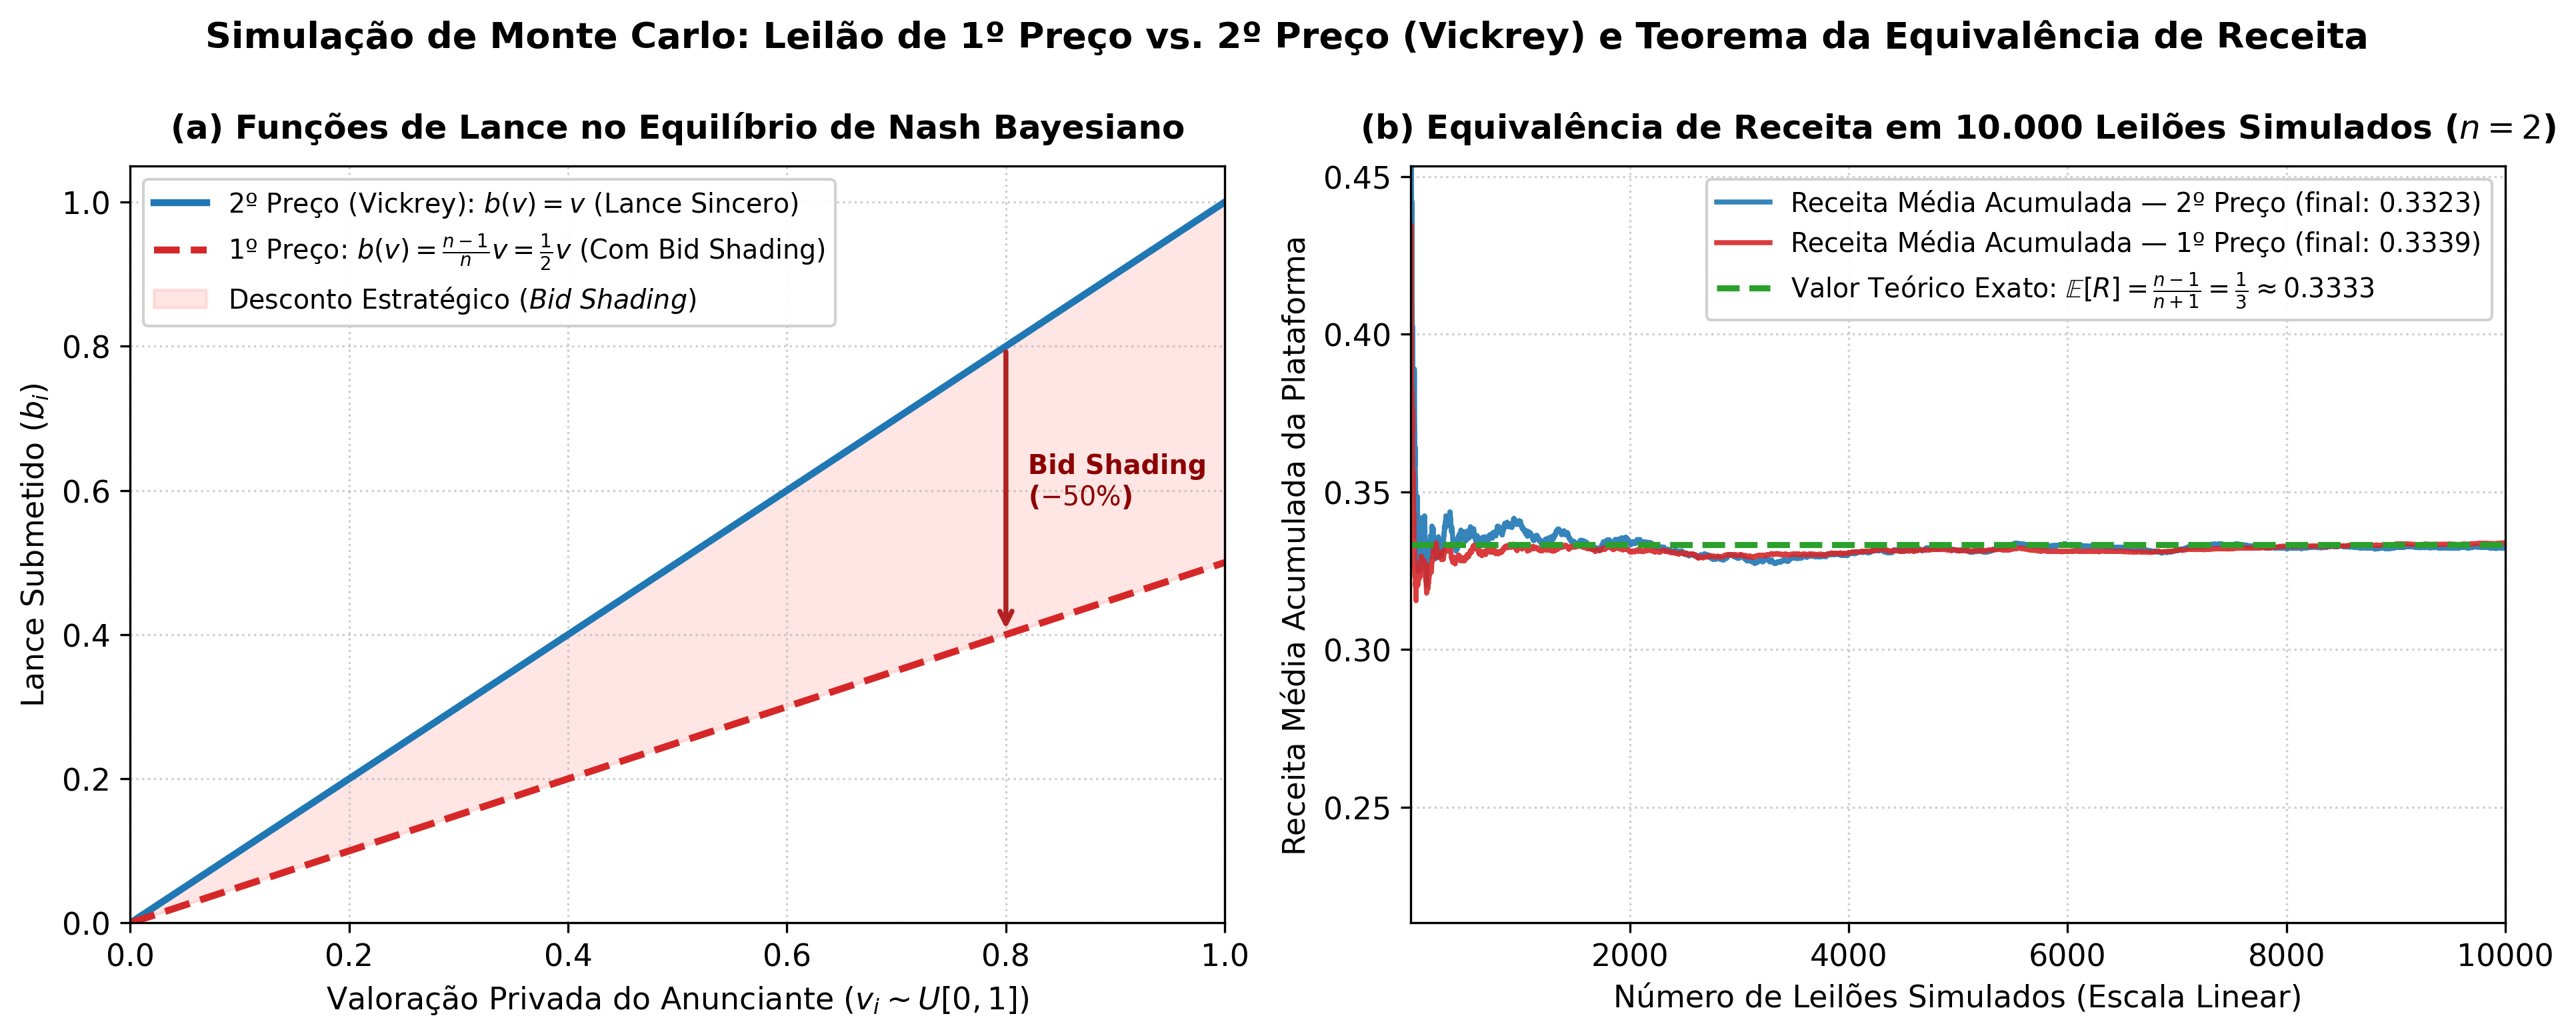
\includegraphics[width=0.75\textwidth]{equivalencia_receita_simulacao.png}
    \par\vspace{0.05cm}
    {\footnotesize Fonte: Elaborado pelos autores (2026).}
    \label{fig:equivalencia_receita}
\end{figure}

Quando a Equivalência de Receita \textbf{quebra} no mundo real \cite[p.~18--26]{klemperer2004}? Quando alguma das Hipóteses (1) a (4) é violada:
\begin{enumerate}[label=\arabic*.]
    \item \textbf{Quebra da Hipótese 3 --- Aversão ao Risco:} Se os compradores têm medo de perder o objeto, no \textbf{1º Preço} eles têm receio de dar um desconto grande e perder por pouco, passando a dar lances mais altos (ex.: $70\%$ do valor em vez de $50\%$). No \textbf{2º Preço}, a estratégia dominante continua sendo $b_i = v_i$. Logo, com compradores avessos ao risco, \textbf{o 1º Preço dá mais receita ao vendedor do que o 2º Preço}!
    \item \textbf{Quebra da Hipótese 2 --- Assimetria entre Jogadores:} Imagine que disputam um lote de 5G uma \textbf{Operadora Gigante} (valor sempre entre \textbf{R\$\,80~mi e R\$\,100~mi}) e uma \textbf{Operadora Pequena} (valor entre \textbf{R\$\,10~mi e R\$\,75~mi}). No \textbf{Leilão Inglês / 2º Preço}, como cada um vai até $100\%$ do seu valor, a Gigante sempre cobrirá a Pequena ($80 > 75$); sabendo que tem $0\%$ de chance de vencer, a Pequena nem se inscreve e a Gigante leva o lote sozinha pelo preço mínimo! Já no \textbf{1º Preço em Envelope Fechado}, a Gigante (digamos, com valor de R\$\,85~mi) sabe que a rival é fraca e coloca só \textbf{R\$\,50~mi} no envelope para lucrar alto, enquanto a Pequena (que tirou R\$\,70~mi) reduz sua margem e coloca \textbf{R\$\,55~mi}. Isso gera um resultado duplo no 1º Preço: (a) a Pequena tem chance real de vencer ($\text{R\$\,55~mi} > \text{R\$\,50~mi}$), atraindo participantes e aumentando a receita; mas (b) quebra-se a \textbf{Hipótese 4a (Alocação Eficiente)}, pois às vezes a Pequena (valor de R\$\,70~mi) vence a Gigante (valor de R\$\,85~mi)!
    \item \textbf{Conluio / Cartel:} Leilões abertos (inglês) e de 2º preço facilitam que membros de um cartel vigiem e punam na hora quem furar o acordo; já o envelope fechado de 1º preço incentiva a ``traição'' do cartel, gerando maior receita para o leiloeiro.
\end{enumerate}

% =============================================================================
\subsection{Maldição do Vencedor (\textit{Winner's Curse})}
\label{subsec:maldicao_vencedor}

Saindo de Valores Privados e entrando em \textbf{Valor Comum} (Definição~\ref{def:cv}), surge a famosa armadilha informacional:

\begin{definicao}[Maldição do Vencedor --- \textit{Winner's Curse}]
\label{def:maldicao_vencedor}
Em um leilão de \textbf{Valor Comum}, suponha que todos os participantes têm estimativas não-viesadas do valor real $V$ (na média, a estimativa de todos acerta $V$, mas uns erram para mais e outros para menos). Se todos usam a mesma regra de dar lance proporcional à sua estimativa, \textbf{quem ganha o leilão não é quem fez a estimativa mais precisa, mas sim quem cometeu o maior erro de superestimação (o mais otimista da sala)!} Se os jogadores não descontarem esse viés ao calcular seus lances, o vencedor frequentemente pagará mais do que o objeto realmente vale ($p > V$) e terá prejuízo \cite[p.~14]{klemperer2004}.
\end{definicao}

Para visualizar isso, \cite[p.~14 e 53]{klemperer2004} usa a analogia do \textbf{pote de moedas}: imagine um pote de vidro com exatamente \textbf{R\$\,100,00} ($V = 100$) leiloado entre 20 alunos. Na média a turma chuta bem (R\$\,100): uns chutam R\$\,70, outros R\$\,95, outros R\$\,105, e o aluno mais otimista da sala chuta \textbf{R\$\,150}. Se cada um der um lance próximo ao que chutou, quem ganha o leilão é justamente o aluno que achou que tinha R\$\,150; mesmo que ele dê um pequeno desconto e pague R\$\,130, ao abrir o pote descobrirá que só havia R\$\,100 e perderá R\$\,30!

Como um jogador racional evita a Maldição do Vencedor no Equilíbrio de Nash Bayesiano? Aplicando o \textbf{Condicionamento na Vitória}: em vez de perguntar \textit{``quanto vale o poço dado que meu geólogo disse 150 milhões?''}, ele pergunta: \textit{``quanto vale o poço dado que meu geólogo disse 150 milhões \textbf{E os geólogos de todas as outras 9 empresas disseram menos que 150 milhões}?''} ($\mathbb{E}[V \mid s_i, \max_{j \neq i} s_j < s_i]$). Por isso, quanto maior o número de concorrentes num leilão de valor comum, mais conservador (menor) deve ser o lance!

\section{Modelo Resolvido}
\label{sec:modelo_resolvido}

Resolvemos a seguir, passo a passo, o modelo de leilão de primeiro preço com dois participantes e valores uniformes entre $0$ e $1$ \cite[p.~15--17]{vickrey1961}, comparando sua receita com a do leilão de segundo preço \cite[Apêndice~1.D, p.~48]{klemperer2004}.

\subsection{Enunciado}
\label{subsec:enunciado_modelo}

\begin{itemize}
    \item \textbf{Jogadores:} $N = \{1, 2\}$ (dois compradores neutros ao risco).
    \item \textbf{Tipos / Valorações ($v_1, v_2$):} Cada jogador $i$ conhece seu valor privado $v_i$, sorteado de forma independente da distribuição uniforme no intervalo $[0, 1]$ ($v_i \sim U[0, 1]$). Propriedade crucial da uniforme em $[0, 1]$: para qualquer $x \in [0, 1]$, a probabilidade de uma variável uniforme ser menor que $x$ é o próprio $x$, isto é, $\mathbb{P}(v_2 < x) = x$.
    \item \textbf{Ações:} Lances em envelope fechado $b_1 \ge 0$ e $b_2 \ge 0$. Quem der o maior lance vence o objeto (pagando o próprio lance $b_i$ no 1º Preço, ou pagando o lance do concorrente no 2º Preço).
\end{itemize}

\subsection{Solução Completa (Passo a Passo)}
\label{subsec:solucao_passo_a_passo}

Queremos encontrar a estratégia simétrica de Equilíbrio de Nash Bayesiano $\beta(v_i)$ --- a função estritamente crescente e diferenciável (com $\beta(0) = 0$) que indica quanto ofertar no \textbf{Leilão de 1º Preço} quando o valor privado é $v_i$:

\begin{enumerate}[label=\arabic*.]
    \item \textbf{Probabilidade de vitória:} Suponha que o Jogador~$2$ siga a função de equilíbrio $b_2 = \beta(v_2)$. Se o Jogador~$1$ (com valor $v_1$) escolher dar um lance $b_1$, ele vence se $\beta(v_2) < b_1 \iff v_2 < \beta^{-1}(b_1)$. Como $v_2 \sim U[0, 1]$, para todo $b_1 \in [0, \beta(1)]$ (onde $0 \le \beta^{-1}(b_1) \le 1$), a probabilidade de $v_2$ ser menor que $\beta^{-1}(b_1)$ é o próprio $\beta^{-1}(b_1)$:
    \begin{equation}
    \mathbb{P}\big(\beta(v_2) < b_1\big) = \mathbb{P}\big(v_2 < \beta^{-1}(b_1)\big) = \beta^{-1}(b_1).
    \end{equation}
    \textit{Por que podemos ignorar o caso em que $\beta^{-1}(b_1) > 1$ (ou seja, $b_1 > \beta(1)$)?} Porque, como o valor do Jogador~$2$ nunca passa de~$1$ ($v_2 \in [0, 1]$) e $\beta(\cdot)$ é crescente, o \textbf{maior lance possível} que o Jogador~$2$ pode dar no melhor cenário ($v_2 = 1$) é $\beta(1)$. Se o Jogador~$1$ der um lance igual a $b_1 = \beta(1)$ (onde $\beta^{-1}(b_1) = 1$), ele \textbf{já ganha o leilão com $100\%$ de certeza ($\mathbb{P} = 1$)}! Escolher qualquer lance $b_1 > \beta(1)$ manteria a chance de ganhar travada em $100\%$, mas faria o Jogador~$1$ pagar mais caro à toa, reduzindo seu lucro $(v_1 - b_1)$. Logo, qualquer lance $b_1 > \beta(1)$ é estritamente dominado por $\beta(1)$, e todo jogador racional escolhe $b_1 \le \beta(1) \iff \beta^{-1}(b_1) \le 1$.

    \item \textbf{Valor Esperado do Ganho (\textit{Payoff} Esperado) do Jogador 1:}
    \begin{equation}
    \Pi_1(b_1) = (v_1 - b_1)\cdot \mathbb{P}\big(\beta(v_2) < b_1\big) = (v_1 - b_1)\beta^{-1}(b_1).
    \end{equation}

    \item \textbf{Condição de Primeira Ordem (Maximizando em relação a $b_1$):} Derivando $\Pi_1(b_1)$ em relação a $b_1$ pela regra do produto e igualando a zero:
    \begin{equation}
    \frac{d\Pi_1}{db_1} = -\beta^{-1}(b_1) + (v_1 - b_1)\frac{d}{db_1}\!\big[\beta^{-1}(b_1)\big] = 0.
    \end{equation}
    Pelo teorema da derivada da função inversa, no ponto de equilíbrio em que o Jogador~$1$ também usa a estratégia ótima $b_1 = \beta(v_1)$, temos $\beta^{-1}(b_1) = v_1$ e $\frac{d}{db_1}[\beta^{-1}(b_1)] = \frac{1}{\beta'(v_1)}$. Substituindo na equação:
    \begin{equation}
    -v_1 + \frac{v_1 - \beta(v_1)}{\beta'(v_1)} = 0 \implies v_1 \beta'(v_1) + \beta(v_1) = v_1.
    \end{equation}

    \item \textbf{Resolvendo a Equação Diferencial:} O lado esquerdo $v_1 \beta'(v_1) + 1 \cdot \beta(v_1)$ é exatamente a derivada do produto $\frac{d}{dv_1}[v_1 \beta(v_1)]$, o que fornece o lance de equilíbrio\footnote{Generalização: com $n$ jogadores uniformes em $[0, 1]$, \cite[p.~17]{vickrey1961} mostra que o lance de equilíbrio no 1º preço é $b^*(v_i) = \frac{n-1}{n}v_i$: com $n=2$ oferta-se $\frac{1}{2}v_i$; com $n=3$, $\frac{2}{3}v_i$; com $n=10$, $\frac{9}{10}v_i$; quando $n \to \infty$, o lance tende a $100\%$ do valor.}:
    \begin{equation}
    \frac{d}{dv_1}\!\big[v_1 \beta(v_1)\big] = v_1 \implies v_1 \beta(v_1) = \int_0^{v_1} x\, dx = \frac{v_1^2}{2} \implies \boxed{b_{\text{1º}}^*(v_i) = \beta(v_i) = \frac{v_i}{2}.}
    \end{equation}
\end{enumerate}

\subsection{Comparação da Receita Esperada e Interpretação}
\label{subsec:interpretacao_modelo}

Mostramos agora por que o vendedor ganha \textbf{exatamente $\frac{1}{3}$ em média} nos dois formatos:
\begin{enumerate}[label=\arabic*.]
    \item \textbf{Receita Esperada no Leilão de 1º Preço ($\mathbb{E}[R_{\text{1º}}]$):} Quem ganha é o jogador de maior valor, $\max\{v_1, v_2\}$, pagando metade desse valor: $R_{\text{1º}} = \max\{b^*(v_1), b^*(v_2)\} = \frac{1}{2}\max\{v_1, v_2\}$. Como a probabilidade de duas uniformes independentes serem menores que $y$ é $F_{\max}(y) = \mathbb{P}(v_1 \le y)\mathbb{P}(v_2 \le y) = y^2$, a densidade do máximo é $f_{\max}(y) = (y^2)' = 2y$, e a média do máximo é:
    \begin{equation}
    \mathbb{E}[\max\{v_1, v_2\}] = \int_0^1 y \cdot (2y)\, dy = \left[\frac{2y^3}{3}\right]_0^1 = \frac{2}{3} \implies \boxed{\mathbb{E}[R_{\text{1º}}] = \frac{1}{2} \times \frac{2}{3} = \frac{1}{3}.}
    \end{equation}

    \item \textbf{Receita Esperada no Leilão de 2º Preço / Vickrey ($\mathbb{E}[R_{\text{2º}}]$):} No 2º preço, a estratégia dominante é $b^*(v_i) = v_i$. Vence o maior valor ($\max\{v_1, v_2\}$), mas paga o lance do 2º colocado, que entre 2 jogadores é o menor dos dois valores ($R_{\text{2º}} = \min\{v_1, v_2\}$). Como $\min\{v_1, v_2\} + \max\{v_1, v_2\} = v_1 + v_2$ e $\mathbb{E}[v_1 + v_2] = \frac{1}{2} + \frac{1}{2} = 1$, temos diretamente\footnote{Intuição geométrica \cite[p.~48]{klemperer2004}: $n$ sorteios uniformes em $[0, 1]$ dividem o intervalo em $n+1$ partes iguais em média. Para $n=2$, os valores dividem $[0, 1]$ em três terços ($\mathbb{E}[\min] = 1/3$ e $\mathbb{E}[\max] = 2/3$): no 2º Preço o vendedor recebe o menor valor ($1/3$), e no 1º Preço recebe metade do maior ($\frac{1}{2} \times \frac{2}{3} = 1/3$).}:
    \begin{equation}
    \mathbb{E}[\min\{v_1, v_2\}] = \mathbb{E}[v_1 + v_2] - \mathbb{E}[\max\{v_1, v_2\}] = 1 - \frac{2}{3} = \frac{1}{3} \implies \boxed{\mathbb{E}[R_{\text{2º}}] = \frac{1}{3} = \mathbb{E}[R_{\text{1º}}].}
    \end{equation}
\end{enumerate}

\section{Caso Real: Leilões de Anúncios Online (Google Ads e \textit{Ad Exchanges})}
\label{sec:caso_real}

\subsection{Definições Prévias e Evolução Histórica (\texorpdfstring{1º Preço $\to$ 2º Preço $\to$ 1º Preço}{1º Preço para 2º Preço para 1º Preço})}
\label{subsec:descricao_caso}

Antes de analisarmos o mercado de anúncios digitais, definimos quatro termos básicos do setor:
\begin{itemize}
    \item \textbf{Impressão (\textit{Impression}):} Cada vez que uma página ou busca carrega e exibe um espaço publicitário para um usuário (disparando um leilão instantâneo em menos de $100$ milissegundos).
    \item \textbf{CTR (\textit{Click-Through Rate} --- Taxa de Cliques):} Probabilidade (entre $0$ e $1$, ou em $\%$) de o usuário clicar no anúncio caso ele seja exibido (ex.: $\text{CTR} = 5\%$ significa $5$ cliques a cada $100$ exibições).
    \item \textbf{CPC (\textit{Cost Per Click} --- Custo por Clique):} Modalidade em que o anunciante só paga à plataforma se o usuário efetivamente clicar no anúncio \cite{edelman2007,varian2007}.
    \item \textbf{CPM (\textit{Cost Per Mille} --- Custo por Mil Impressões):} Modalidade usada em \textit{banners} (\textit{Ad Exchanges}) na qual o anunciante paga pela simples exibição do anúncio na tela \cite{despotakis2021}.
\end{itemize}

A história desse mercado divide-se em \textbf{duas grandes fases} que conectam todos os conceitos deste trabalho: (1) a \textbf{Fase 1 (1997--2018)}, quando o mercado abandonou o 1º Preço pioneiro da \textit{Overture/Yahoo} e migrou em 2002 para o \textbf{2º Preço} (GSP na busca do Google Ads e Vickrey puro no Google AdX) \cite{edelman2007,varian2007}; e (2) a \textbf{Fase 2 (2019--Presente)}, quando o Google Ad Manager e as \textit{Ad Exchanges} abandonaram o 2º Preço e voltaram ao \textbf{Leilão de 1º Preço} com algoritmos de \textit{Bid Shading} \cite{despotakis2021}.

\subsubsection{A Primeira Mudança (2002): Do 1º para o 2º Preço (O Ciclo em ``Dente de Serra'')}

Entre 1997 e 2001, na plataforma pioneira \textit{Overture}, o leilão era de \textbf{1º Preço} (quem vencesse pagava o próprio lance), mas os anunciantes podiam ver na tela quanto o concorrente estava ofertando e mudar o lance a qualquer segundo \cite[p.~245--246]{edelman2007}. Imagine dois anunciantes disputando o 1º lugar da busca: para a \textbf{Nike}, o clique vale até $v_{\text{Nike}} = \text{R\$\,10,00}$; para a \textbf{Adidas}, vale até $v_{\text{Adidas}} = \text{R\$\,5,00}$. Como era 1º Preço, cada um queria pagar apenas R\$\,0,01 a mais que o rival:
\begin{enumerate}[label=\arabic*.]
    \item A Adidas começa dando \textbf{R\$\,1,00}. O robô da Nike vê isso e muda seu lance para \textbf{R\$\,1,01};
    \item Segundos depois, o robô da Adidas (que aguenta ir até R\$\,5,00) sobe para \textbf{R\$\,1,02}; a Nike sobe para \textbf{R\$\,1,03}, e ambos sobem de centavo em centavo até a Adidas atingir seu limite (\textbf{R\$\,5,00}) e a Nike cobrir com \textbf{R\$\,5,01};
    \item \textbf{Mas o ciclo não parava em R\$\,5,01!} Quando a Nike assumia o topo por R\$\,5,01, a Adidas via que não conseguia mais vencer o 1º lugar e \textbf{derrubava seu lance de volta para o mínimo (R\$\,1,00)} para ficar em 2º lugar pagando barato;
    \item No segundo seguinte, o robô da Nike via que a Adidas estava oferecendo só R\$\,1,00, percebia que estava pagando R\$\,5,01 à toa e \textbf{baixava seu lance para R\$\,1,01} --- fazendo a Adidas voltar a subir para R\$\,1,02 e reiniciando a escadinha $24$ horas por dia!
\end{enumerate}

Esse padrão em \textbf{``dente de serra'' (\textit{sawtooth})} sobrecarregava servidores, gerava gastos inúteis com robôs de contraespeculação \cite[p.~20]{vickrey1961} e reduzia a receita do buscador (pois durante a subida da escadinha a Adidas ficava em 1º lugar metade do tempo pagando barato). Em \textbf{2002}, o Google resolveu isso adotando o \textbf{2º Preço}: a Nike escreve \textbf{R\$\,10,00} uma única vez, a Adidas escreve \textbf{R\$\,5,00} uma única vez, e o próprio sistema do Google cobra automaticamente da Nike o lance da Adidas mais 1 centavo (\textbf{R\$\,5,01}), estabilizando o mercado \cite[p.~246]{edelman2007}.

\subsubsection{A Segunda Mudança (2019): Por que o Mercado Voltou do 2º para o 1º Preço?}

Por que então as corretoras de \textit{banners} (\textit{Ad Exchanges}) e o Google Ad Manager decidiram voltar para o \textbf{1º Preço} em 2019? Segundo \cite{despotakis2021}, dois problemas práticos destruíram o 2º Preço nos \textit{banners}:

\paragraph{Motivo 1 --- A ``Trapaça do Leiloeiro'' no 2º Preço (Preços Mínimos Ocultos / \textit{Soft Floors}):}
No 2º Preço, a Nike entrega seu valor máximo verdadeiro no envelope (\textbf{R\$\,10,00}) e a Adidas entrega \textbf{R\$\,2,00}; pela regra honesta, a Nike deveria pagar R\$\,2,00. Porém, ao abrir os envelopes e ver que a Nike topava pagar R\$\,10,00, muitas corretoras usavam ``preços mínimos ocultos de última hora'' (\textit{soft floors}): inventavam um piso de reserva de \textbf{R\$\,8,50} depois de espiar o lance da Nike e cobravam R\$\,8,50 dela \cite[p.~3]{despotakis2021}! Como o leilão era fechado no servidor da corretora, a Nike não tinha como auditar se existiu mesmo outro lance de R\$\,8,50. No \textbf{1º Preço}, isso acaba na hora: se a Nike escreve \textbf{R\$\,5,00} e ganha, ela paga exatamente os R\$\,5,00 que ela mesma escreveu.

\paragraph{Motivo 2 --- O ``Torneio de Duas Etapas'' (\textit{Header Bidding}):}
Os sites de notícias perceberam que ganhavam mais dinheiro colocando \textbf{duas ou mais corretoras para competir ao mesmo tempo} pelo mesmo \textit{banner} (ex.: \textbf{Corretora~A} contra \textbf{Corretora~B}), criando um \textbf{Torneio de 2 Etapas} \cite[p.~2--4]{despotakis2021}: na \textbf{Etapa~1 (Semifinal dentro de cada Corretora)}, cada corretora faz um leilão entre seus clientes e manda o valor vencedor para a Final; na \textbf{Etapa~2 (Grande Final no Site de Notícias)}, quem mandou o número maior leva o \textit{banner}. Veja o desastre quando a Corretora~A usava \textbf{2º Preço} na Semifinal:
\begin{itemize}
    \item \textbf{Na Semifinal da Corretora~A (2º Preço):} A \textbf{Nike} dá \textbf{R\$\,10,00} e a \textbf{Adidas} dá \textbf{R\$\,2,00}. A Nike vence a semifinal, mas pela regra de 2º Preço seu preço cai imediatamente para o lance da Adidas (\textbf{R\$\,2,00}). A Corretora~A envia apenas \textbf{R\$\,2,00} para a Grande Final!
    \item \textbf{Na Semifinal da Corretora~B (1º Preço):} A \textbf{Puma} dá lance de \textbf{R\$\,6,00}, vence, e a Corretora~B envia \textbf{R\$\,6,00} para a Grande Final.
    \item \textbf{Na Grande Final do Site de Notícias (R\$\,2,00 vs. R\$\,6,00):} \textbf{A Puma (com R\$\,6,00) derrota a Nike (que estava disposta a pagar R\$\,10,00)!} A regra de 2º Preço da Corretora~A reduziu o lance da Nike cedo demais (na semifinal), fazendo-a perder a Final!
\end{itemize}
Para que seus anunciantes parassem de perder na Final e a cobrança ficasse transparente, todas as corretoras --- encerrando com o Google em 2019 --- migraram para o \textbf{Leilão de 1º Preço} \cite[Proposição~4, p.~22]{despotakis2021}: agora, se a Nike dá um lance (com \textit{bid shading}) de R\$\,7,00 na Corretora~A, esse número vai inteiro (R\$\,7,00) até a Final e derrota os R\$\,6,00 da Puma!

% =============================================================================
\subsection{Modelagem como Jogo Bayesiano}
\label{subsec:modelagem_caso}

Traduzimos formalmente o leilão de anúncios online nos 4 elementos de um Jogo Bayesiano:
\begin{enumerate}[label=\arabic*.]
    \item \textbf{Jogadores ($N = \{1, 2, \dots, n\}$):} Os $n$ anunciantes concorrentes (ex.: Nike, Adidas, Puma) que disputam em tempo real um espaço publicitário na tela de um usuário.
    \item \textbf{Tipos e Informação Disponível ($v_i$ e $F$):} O \textbf{Tipo ($v_i$)} de cada anunciante é o valor monetário máximo (em R\$) que $1$ clique daquele usuário vale para ele. Na prática, se a Nike vende um tênis com \textbf{R\$\,200,00 de lucro líquido} e $1$ a cada $20$ pessoas que clicam no anúncio efetivamente compra o tênis (chance de conversão de $5\%$), então $1$ clique vale em média:
    \begin{equation}
    v_{\text{Nike}} = \underbrace{5\%}_{\text{Chance de conversão}} \times \underbrace{\text{R\$\,200,00}}_{\text{Lucro por venda}} = \textbf{R\$\,10,00 por clique}.
    \end{equation}
    É um jogo bayesiano porque $v_i$ é \textbf{Informação Privada} (só a Nike conhece sua margem de lucro e sua taxa de conversão internas), enquanto as regras do leilão e a distribuição estatística geral de mercado $F(v)$ dos concorrentes formam o \textbf{\textit{Prior} Comum}.
    \item \textbf{Estratégias ($b_i(v_i)$):} Função que transforma o valor privado $v_i$ em um lance $b_i \ge 0$. Na \textbf{Fase~1 (2º Preço / Vickrey)}, a estratégia ótima é a revelação sincera $b_i^*(v_i) = v_i$. Na \textbf{Fase~2 (1º Preço após 2019)}, a estratégia ótima em ENB é aplicar \textit{Bid Shading}: $b_i^*(v_i) = \mathbb{E}[\max_{j \neq i} v_j \mid \max_{j \neq i} v_j < v_i] = \frac{n-1}{n}v_i < v_i$.
    \item \textbf{Funções de \textit{Payoff} ($u_i$):} Se o anunciante perde ($b_i < \max_{j \neq i} b_j$), ganha $u_i = 0$. Se vence ($b_i > \max_{j \neq i} b_j$) e recebe o clique, seu ganho por clique no \textbf{2º Preço} ($p = \max_{j \neq i} b_j$) e no \textbf{1º Preço} ($p = b_i$) é:
    \begin{equation}
    u_i^{\text{2º Preço}} =
    \begin{cases}
        v_i - \max\limits_{j \neq i} b_j, & \text{se } b_i > \max\limits_{j \neq i} b_j, \\
        0, & \text{se } b_i < \max\limits_{j \neq i} b_j;
    \end{cases}
    \qquad
    u_i^{\text{1º Preço}} =
    \begin{cases}
        v_i - b_i, & \text{se } b_i > \max\limits_{j \neq i} b_j, \\
        0, & \text{se } b_i < \max\limits_{j \neq i} b_j.
    \end{cases}
    \end{equation}
    \textit{Onde entra o CTR no Payoff?} Antes de saber se o usuário vai clicar ou não no anúncio exibido, basta multiplicar o lucro de 1 clique $(v_i - p)$ pela probabilidade de clique: $\text{Payoff Esperado por Exibição} = \text{CTR} \times (v_i - p)$. Como $\text{CTR} > 0$ é uma constante positiva, maximizar $\text{CTR} \times (v_i - p)$ gera exatamente o mesmo lance ótimo que maximizar $(v_i - p)$ \cite[p.~1164]{varian2007}.
\end{enumerate}

\section{Ligação com o Curso}
\label{sec:ligacao_curso}

O estudo dos leilões como jogos bayesianos complementa o conteúdo da disciplina \textbf{GED-62 --- Teoria dos Jogos} em cinco pontos centrais:

\begin{enumerate}[label=\arabic*.]
    \item \textbf{Superação da Hipótese de Informação Completa:} Nos jogos matriciais clássicos estudados no início do curso (como o Dilema dos Prisioneiros, a Batalha dos Sexos e o modelo de Cournot com custos conhecidos), cada jogador conhece exatamente os \textit{payoffs} do oponente. Os leilões mostram como aplicar a Teoria dos Jogos quando \textbf{há segredo sobre quanto o adversário valoriza o prêmio}, utilizando a Transformação de Harsanyi, na qual a Natureza sorteia os tipos privados \cite{harsanyi1967,gibbons1992}.
    \item \textbf{Estratégia como Função (e não ponto isolado):} Em vez de escolher uma única linha ou coluna de uma matriz, a estratégia no equilíbrio bayesiano é uma função contínua $b_i(v_i)$ que define uma ação para cada um dos infinitos tipos possíveis.
    \item \textbf{Contraste entre Dominância e Equilíbrio de Nash Bayesiano:}
    \begin{itemize}
        \item O \textbf{Leilão de 2º Preço (Vickrey)} resgata o conceito mais forte visto no início do curso: a \textbf{Estratégia Fracamente Dominante} ($b_i = v_i$), que não depende de crenças probabilísticas sobre os rivais, pois todas as demais estratégias $b_i \neq v_i$ são \textbf{Estratégias Fracamente Dominadas} (isto é, estratégias que nunca proporcionam um ganho maior do que $b_i = v_i$ em nenhum cenário e geram um ganho estritamente menor em pelo menos um cenário dos adversários) \cite[p.~20]{vickrey1961}.
        \item O \textbf{Leilão de 1º Preço}, por outro lado, exige um \textbf{Equilíbrio de Nash Bayesiano} ($b_i = v_i/2$), que depende crucialmente da distribuição de probabilidade $F$ dos tipos rivais.
    \end{itemize}
    \item \textbf{Jogos Dinâmicos vs.\ Estáticos (Equivalência Estratégica):} Conecta os jogos sequenciais em forma extensiva (Leilão Inglês ascendente e Leilão Holandês descendente) com os jogos simultâneos em forma normal (Leilões em Envelope Fechado de 2º e de 1º Preço).
    \item \textbf{Teoria dos Jogos Reversa (Desenho de Mecanismos):} Em vez de apenas resolver um jogo com regras fixas, o leiloeiro utiliza a Teoria dos Jogos para \textbf{projetar as regras do jogo} (escolha entre 1º e 2º preço, definição de preços de reserva e regras de transparência) de modo a induzir eficiência alocativa ou maximizar a receita esperada \cite{myerson1981,klemperer2004}.
\end{enumerate}

\section{Conclusão}
\label{sec:conclusao}

Neste artigo, estudamos os leilões sob a perspectiva dos jogos bayesianos, mostrando como a Transformação de Harsanyi permite modelar e resolver disputas estratégicas nas quais cada comprador possui informação privada sobre sua disposição a pagar. Partindo dos conceitos de tipo privado, crença a priori comum (\textit{prior} comum), estratégias funcionais e Equilíbrio de Nash Bayesiano, distinguimos os leilões de Valores Privados Independentes dos leilões de Valor Comum, nos quais a vitória sem o devido desconto estatístico expõe o licitante mais otimista à Maldição do Vencedor.

No modelo analítico resolvido para dois licitantes simétricos com valorações uniformes em $[0, 1]$, demonstramos que o Leilão de Primeiro Preço induz um sombreamento de lance (\textit{bid shading}) de $50\%$ ($b^*(v_i) = v_i/2$), enquanto o Leilão de Segundo Preço de Vickrey torna a revelação sincera ($b^*(v_i) = v_i$) uma estratégia fracamente dominante. Comprovamos analiticamente e por meio de uma simulação de Monte Carlo de $10.000$ leilões em Python que ambos os formatos convergem para a mesma receita esperada teórica $\mathbb{E}[R] = \frac{n-1}{n+1} = \frac{1}{3}$, confirmando o Teorema da Equivalência de Receita.

Por fim, o estudo dos leilões de anúncios online (Google Ads e \textit{Ad Exchanges}) ilustrou como a teoria orienta decisões reais da indústria: a migração do primeiro para o segundo preço em 2002 eliminou a instabilidade dos ciclos em dente de serra, enquanto a transição de volta ao primeiro preço em 2019 respondeu à competição simultânea em múltiplos estágios do \textit{Header Bidding} e à busca por transparência, consolidando o uso moderno dos algoritmos de \textit{bid shading}.

\section{Referências da Literatura}
\label{sec:referencias}

\renewcommand{\refname}{}

\begin{thebibliography}{99}

\bibitem[DESPOTAKIS; RAVI; SAYEDI, 2021]{despotakis2021}
DESPOTAKIS, Stylianos; RAVI, R.; SAYEDI, Amin. First-price or second-price? A study of the transition from second-price to first-price auctions in online advertising. \textbf{Management Science}, Catonsville, v. 67, n. 10, p. 6432--6448, out. 2021.

\bibitem[EDELMAN; OSTROVSKY; SCHWARZ, 2007]{edelman2007}
EDELMAN, Benjamin; OSTROVSKY, Michael; SCHWARZ, Michael. Internet advertising and the generalized second-price auction: Selling billions of dollars worth of keywords. \textbf{American Economic Review}, Nashville, v. 97, n. 1, p. 242--259, mar. 2007.

\bibitem[GIBBONS, 1992]{gibbons1992}
GIBBONS, Robert. \textbf{Game theory for applied economists}. Princeton: Princeton University Press, 1992.

\bibitem[HARSANYI, 1967]{harsanyi1967}
HARSANYI, John C. Games with incomplete information played by ``Bayesian'' players, I--III: Part I. The basic model. \textbf{Management Science}, Catonsville, v. 14, n. 3, p. 159--182, nov. 1967.

\bibitem[KLEMPERER, 2004]{klemperer2004}
KLEMPERER, Paul. \textbf{Auctions}: theory and practice. Princeton: Princeton University Press, 2004.

\bibitem[MYERSON, 1981]{myerson1981}
MYERSON, Roger B. Optimal auction design. \textbf{Mathematics of Operations Research}, Catonsville, v. 6, n. 1, p. 58--73, fev. 1981.

\bibitem[VARIAN, 2007]{varian2007}
VARIAN, Hal R. Position auctions. \textbf{International Journal of Industrial Organization}, Amsterdã, v. 25, n. 6, p. 1163--1178, dez. 2007.

\bibitem[VICKREY, 1961]{vickrey1961}
VICKREY, William. Counterspeculation, auctions, and competitive sealed tenders. \textbf{The Journal of Finance}, Nova York, v. 16, n. 1, p. 8--37, mar. 1961.

\end{thebibliography}


\end{document}
